\section{The CPR Toolkit}

The CPR (Comprehensible Provenance Record) Toolkit is a suite of tools for recording, storing, querying, and visualizing the run-time provenance of artifacts produced by a run of a computational workflow. While the primary purpose of CPR  is to automate the monitoring and management of provenance-relevant events and records associated with a Whole Tale \emph{recorded run}, the toolkit can be employed in any Linux-based computing environment.

Figure 1 illustrates the flow of information through elements of the CPR toolkit. CPR employs \programname{ReproZip} to observe system calls invoked as part of the recorded run and to record metadata about (1) the operating-system level processes comprising the overall computation; (2) the files accessed by these processes; and (3) the access mode for file accesses, i.e. whether the process opened the file for reading, writing, or both. ReproZip captures and records all of this information in a SQLite database with a schema specific to ReproZip

\begin{figure}
    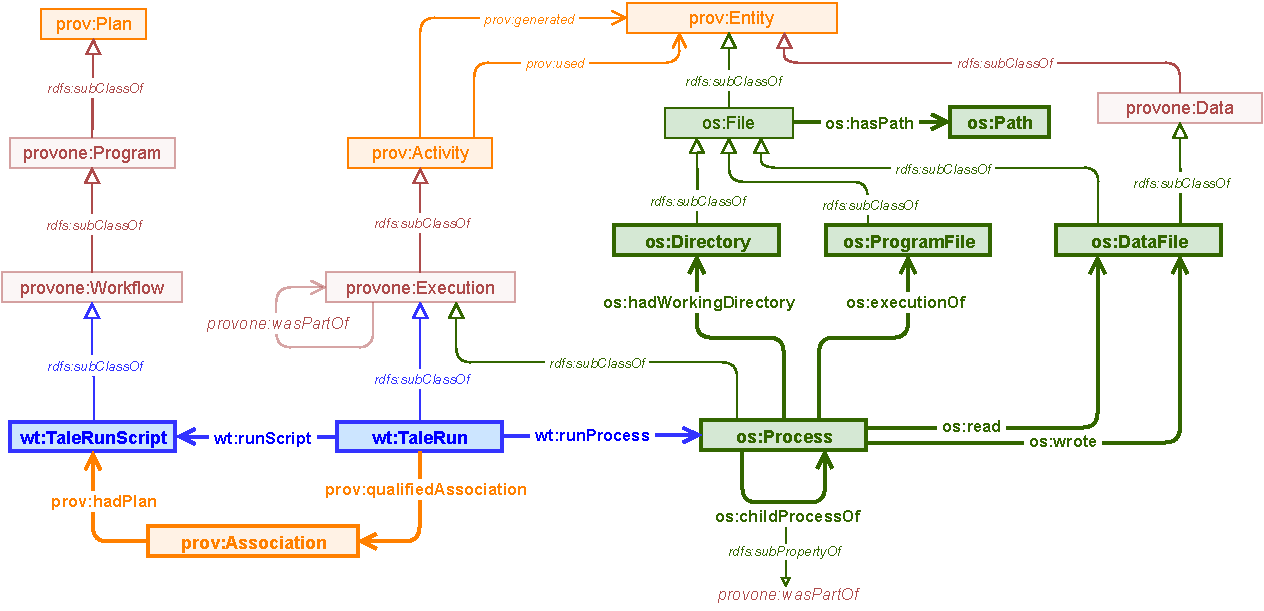
\includegraphics[width=\linewidth]{figures/cpr-vocab.pdf}
    \caption{The CPR vocabulary subclasses terms in the PROV and ProvONE vocabularies.}
    \label{fig:cpr-vocab}
\end{figure}

Once a recorded run is complete, the \programname{cpr} utility extracts these OS-level records from the ReproZip trace, transform them into RDF triples, and loads the triples into an RDF dataset in an instance of Blazegraph. The triples are expressed using a vocabulary developed to represent provenance information in the context of Whole Tale recorded run executions. The CPR vocabulary (Figure \ref{fig:cpr-vocab}) extends PROV and ProvONE with subclasses and new concepts specific to Whole Tale, supporting storage and query of provenance captured from multiple recorded runs and versions of multiple Tales. CPR can represent this vocabulary either as Datalog facts or as RDF triples.

The CPR vocabulary distinguishes between a number of general roles that files accessed during a run may play. A simple YAML file is used to declare prospectively the role of individual files, the contents of particular directories, or of entire directory trees. By using these declarations while converting a ReproZip trace to the CPR vocabulary, CPR is able to distinguish data files of scientific significance from shared libraries provided by the operating system or software dependencies.

Finally, the Geist reporting tool is used to pose SPARQL queries against the Blazegraph instance, to format the query results as reports, and to create visualizations of query results using Graphviz.  Geist queries, reports, and visualizations may be parameterized; in Whole Tale we plan to create a predefined set of reports and visualizations following each recorded run.

